\documentclass[11pt]{scrartcl}
\usepackage{dominatrix}
\usepackage{colortbl}
\usepackage{pgfplots}
\newcommand{\jon}{Jón }
\pgfplotsset{compat=1.9}
\renewcommand\thesubsection{\alph{subsection}}
\definecolor{light-gray}{gray}{0.75}
\title{Mathematics Crash Course}
\subject{ECON W3213 Spring 2014 \jon Steinsson}
\author{Linan Qiu, lq2137}
\begin{document}
\maketitle

\begin{abstract}
This set of recitation notes covers \textbf{Production}. This is in no way a substitute for attending lectures, but just in case you dozed off or checked your boyfriend's Facebook page while \jon was working Calculus magic on the board, this set of notes should save you.
\end{abstract}

\section{Production Function}

Let's say that you're from Insomnialand, and you survive on cookies and only on cookies. We represent the amount of cookies you produce by the letter $Y$. This is your output.

The amount of cookies you produce depend on the amount of machinery (capital) $K$ you have, and the amount of people you slave drive to produce cookies $L$. 

Hence, we say that 

\[Y = F(K,L) \]

You should always think of output in terms of cookies -- so that you remember that we're always talking about \textbf{real output}. Remember \jon always says, "Let's set relative prices to 1." Effectively, he's saying that you price everything relative to that item that costs \$1. Hence, pricing is relative. In other words, if inflation happens, all the prices rise by the same amount, and relative prices don't change. At this stage, this is a good thing to do since we don't want to be bogged down by monetary and inflationary concerns.

The cookie production function can take many forms, for example

\begin{itemize}
	\item $Y = K + L$
	\item $Y = \max (K,L)$
	\item $Y = \min (K,L)$
\end{itemize}

They all have different implications, but the one we're concerned with is the Cobb-Douglas production function because it satisfies a few important properties.

\section{Cobb Douglas Production Function}

The Cobb-Douglas production function is of the form

\[Y = \bar{A} K^\alpha L^{1-\alpha} \]

where $0 < \alpha < 1$. This means that the exponents $\alpha + (1-\alpha) = 1$

$\bar{A}$ is a "collector" constant that represents technology, efficiency, and other things not accounted for by $K$ and $L$. We call this \textbf{Total Factor Productivity}, since it acts as an multiplier to $K^\alpha L^{1-\alpha}$

Let's see what properties it has.

\subsection{Y is Increasing in K and L}

Intuition first. If you increase the number of machines $K$, will you be able to produce more cookies? Of course! What if you increase the amount of labor $L$? Same thing.

We can observe this mathematically as well.

\begin{align*}
\frac{\partial Y}{\partial K} &= \bar{A} (\alpha K^{\alpha - 1}) L^{1-\alpha} > 0 \\ 
\frac{\partial Y}{\partial L} &= \bar{A} K^\alpha ((1-\alpha)L^{-\alpha}) > 0
\end{align*}

The proof that both of these statements are positive is left as an exercise to the reader.

\subsection{Y is Increasing in K and L at a Declining Rate}

Intuition first again. If you keep increasing the number of machines $K$ and \emph{hold labor} $L$ \emph{constant}, you will eventually produce less and less cookies per machine added. Same goes for labor if you \emph{hold capital constant}. Why? Diminishing marginal returns. If you have too many machines but not enough workers, the machines will be idle. If you have too many workers for the machines, they overcrowd. Simple as that.

Mathematically, we say that $Y$ is increasing in $K$, but at a \textbf{declining} rate. $Y$ is also increasing $L$, but at a \textbf{declining} rate.

\begin{figure}[ht!]
\begin{subfigure}[b]{0.5\textwidth}
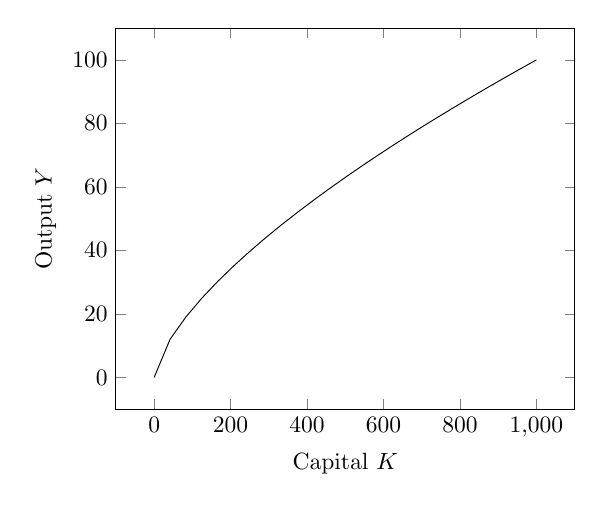
\begin{tikzpicture}[scale=0.85]
\begin{axis}[xlabel={Capital $K$},ylabel={Output $Y$}]
\addplot[domain=0:1000,black]
{(x^(2/3))};
%\addplot[domain=0:1000,black]
%{(x^(1/3))};
\end{axis}
\end{tikzpicture}
\caption{Plot of $Y$ against $K$ holding $L$ constant}
\end{subfigure}
\hspace{2ex}
\begin{subfigure}[b]{0.5\textwidth}
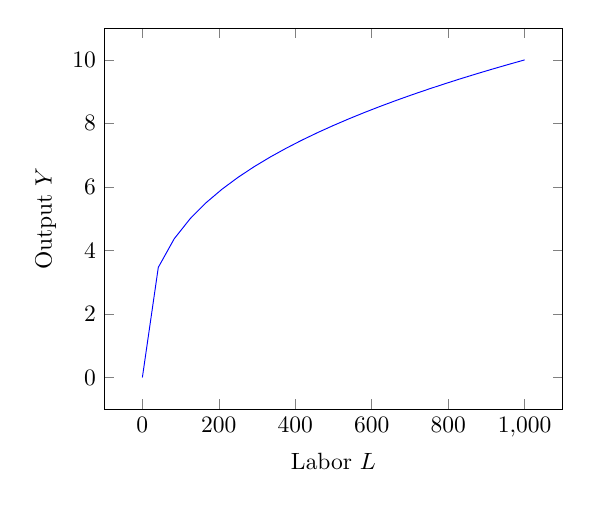
\begin{tikzpicture}[scale=0.85]
\begin{axis}[xlabel={Labor $L$},ylabel={Output $Y$}]
%\addplot[domain=0:1000,black]
%{(x^(2/3))};
\addplot[domain=0:1000,blue]
{(x^(1/3))};
\end{axis}
\end{tikzpicture}
\caption{Plot of $Y$ against $L$ holding $K$ constant}
\end{subfigure}
\caption{Y Increasing in K and L at a Declining Rate}
\end{figure}

This requires us to find the second derivatives.

\begin{align*}
\frac{\partial^2 Y} {\partial K^2} &= \bar{A} (\alpha (\alpha - 1) K^{\alpha - 2}) L^{1-\alpha} < 0\\
\frac{\partial^2 Y}{\partial L^2} &= \bar{A} K^\alpha ((1-\alpha)(-\alpha)L^{-\alpha -1}) < 0
\end{align*}

\begin{itemize}
	\item $\frac{\partial^2 Y} {\partial K^2}  < 0$ because $(\alpha - 1)$ is negative, since we stipulated that $0 < \alpha < 1$. 
	\item $\frac{\partial^2 Y}{\partial L^2} < 0$ because $(1-\alpha)$ is negative.
\end{itemize}

\subsection{Constant Returns to Scale}

Returns to scale is \textbf{different} from Diminishing Marginal Returns. Return to scale answers the question, "If I increase \emph{all} inputs by the same proportion, what will happen to output?"

In other words, we're taking our original $K$ and $L$, and multiplying them both by the same proportion $c$. Then we investigate what happens to output.

So originally, we have

\[Y_0 = \bar{A} K^\alpha L^{1-\alpha} \]

After increases in input, we have

\begin{align*}
Y_1 &= \bar{A} (cK)^\alpha (cL)^{1-\alpha} \\
&= \bar{A} (c^\alpha)(K)^\alpha (c^{1-\alpha})(L)^{1-\alpha} \\
&= c\bar{A} K^\alpha L^{1-\alpha} \\
&= cY_0
\end{align*}

We have just shown that if I increase both $K$ and $L$ by $c$, then $Y$ gets increased by the same factor.

This is what we mean by \textbf{Constant Returns to Scale}

\section{Firms' Optimal Choice}

\subsection{Optimal Choice of Capital}

\subsection{Optimal Choice of Labor}

\section{Share of Output}






\end{document}